\section{Technical Preliminaries}
\label{sec:summary}
%This section explains at a high level our proof techniques and the road-map of the proofs.
In this section, we present some useful preliminary results and ideas for  proving the impossibility results, by showing existence of certain contradictory executions.
In each proof, we use a simple system consisting of two servers, $s_x$ and $s_y$, denote the stored values as $x$ and $y$, respectively, and either two or three clients.
One of the clients is a writer $w$, which initiates only \wots{}.
One or two of the clients are readers, $r_1$ and $r_2$, which initiate only \rots{}.

%{ \color{blue} 
{\bf Client-to-client (C2C) communication.}
We consider two types of settings pertinent to communication among the clients: $(i)$ allow C2C communication, where a client can send a message to any other client, and $(ii)$ disallow C2C communications, where a client cannot send any message directly to another client in the system.
%}

%\wl{Note, i tried to unify definition above so it can be used in 5 and 6.1 and need not be repeated.}

Servers $s_x$ and $s_y$ store values for objects $o_x$ and $o_y$, respectively.
%the values  in $o_1$ and $o_2$ belong to the domains $V_1$ and $V_2$, respectively;
the initial values of $o_x$ and $o_y$ are $x_0$ and $y_0$, respectively. Because there is one  object on each server  the server and object identifiers are often used interchangeably to remove redundancy. For instance, we simply say that $s_x$ returns $x_0$ to the client that initiated the transaction, which means that $s_x$ returns the value $x_0$ of object $o_x$ at the end of the READ transaction.  
%We denote the automata for servers $s_x$ and $s_y$ by $s_x$ and $s_y$, respectively, and the automata for the clients  $r_1$, $r_2$ and $w$ by $r_1$, $r_2$  and $w$, respectively.   
% We denote by $S_1$  the subsystem consisting of $s_x$, $s_y$, $r_1$ and $w$,  and  by $S_1$  the  automata composed of  $s_x$, $s_y$, $r_1$ and $w$, i.e., $s_x \times s_y \times w$. 
% Also, we  denote by $\mathcal{A}$,  the automaton representing the entire system consisting of $S_1$ and $r_2$ (i.e., $s_x \times  s_y$  $\times$ $r_1$ $ \times w$ $ \times r_2$). 
 %We assume that between any pair of processes $p_1$ and $p_2$,   such that $p_1 \neq p_2$,   there are channel automata $Channel_{p_1, p_2}$ and $Channel_{p_2, p_1}$.
%Again, with abuse of notation we denote by $\mathcal{S}$ the automata composed of the automatons $s_x$, $s_y$ and $w$. Also, by $\mathcal{T}$ we denote the composition of automaton $\mathcal{S}$ and $r$, i.e., represents the entire system.  
%We used the notation $\writeop{o}{v}$ to mean a write operation with value $v$ on object $o$; and similarly, by $\readop{o}$ we mean a read operation on $o$.
%We  denote by $S_2$ the system, and also the  composed automaton,  consisting of  $s_x$, $s_y$, $r$ and  $w$, by composing the automatons $S_1$ and $r$, i.e., the automaton $S_1 \times r$.
%
%Here, we consider only fair  executions of ${\mathcal A}$.
%For the purpose of proving by contradiction, we  also assume that  any fair execution of $\mathcal{A}$  respects  the SNOW properties. 
 %Also, we assume that in any execution  of $\mathcal{A}$  we can identify each transaction with a unique identifier.
 %Also, we  denote by $\mathcal{A}$, which can also be interpreted as the algorithm, the automaton representing the entire system consisting of $S_1$ and $r$ (i.e., $s_x \times  s_y$ $ \times w$ $ \times r$).

%``All finite executions are fair and in every infinite fair execution all processes takes steps infinitely often.''
%\hl{I commented out the informal def of fair executions here. It's currently not helpful. We either need a formal def of it or omit it for not making it come back to us. No previous reviews questioned it either. I propose not defining it and even take out fair executions from later proofs.}
\remove{
\sloppy Consider an execution of ${\mathcal A}$ with  three transactions: a \wot{} $W \equiv $ $WRITE($$ (o_1, x_1),  (o_2, y_1) )$ initiated by  $w$, where $x_1 \neq x_0$ and $y_1 \neq y_0$; and  \rots{} $R_1 \equiv READ$$(o_1, o_2)$  and   $R_2 \equiv READ$$(o_1, o_2)$
 initiated by $r_1$ and $r_2$, respectively.  Let us denote by 
$op_1^r$ and $op_2^r$  the read operations of types $\readop{o_1}$ and  $ \readop{o_2} $, respectively. Any distributed algorithm $\mathcal{A}$ in this setting can be represented by the composition of the individual process and channel automatons. 
}
\remove{
Now we describe the set of actions corresponding to the  \rots{} in a fair execution $\epsilon$ of $\mathcal{A}$. 
%Consider an arbitrary execution $e$ of $\mathcal{A}$ where $R$ is a \rot{} and $W$ is a \wot{}.
 %During the execution of $R$,  in $\epsilon$, each of  the read operations $op_1^r$ and $op_2^r$ in  $R$  is associated  with a sequence of external actions.
   Clearly,  in $\epsilon$, the actions $\inv{op_i^r}$ and $\resp{op_i^r}$ appear between the actions $\INV{R}$ and $\RESP{R}$. The  action  $\inv{op_i^r}$ is followed by action $send(m_i^r)_{r, s_i}$, which is 
 for  sending  the read object value request to server $s_i$. This request $m_i^r$ is communicated to $s_i$, via the channel automaton $Channel_{r, s_i}$.  Automaton 
 $s_i$ eventually receives the request 
  via the action   
   $recv(m_i^r)_{r, s_i}$,  and subsequently, responds back to $r$, with object value $v_i$,  through the action $send(v_i)_{s_i, r}$.  Next, 
   value $v_i$, $v_i \in V_i$,  communicated by the automaton  $Channel_{s_i, r}$,  is 
received at $r$ via the action  $recv(v_i)_{s_i, r}$, and finally,  $op_i^r$ completes with  response action $\resp{op_i^r}$ and returns $v_i$ to $r$. 
}

Our proofs often use a special type of execution fragment, named non-blocking fragments, that represent the \rot{} algorithm is non-blocking and returns one version of each object. The one-round property is captured by allowing only one non-blocking fragment on each server for a \rot{}. Our proof strategy plays non-blocking fragments against the requirements of strict serializability and write isolation under the freedom of network asynchrony. We explain non-blocking fragments and helper notations in the context of execution $\alpha$, of the system described as above, as follows:

%Due to the wait-free requirement for  the \wots{}, $W$ completes, and we denote by $\INV{W}$ the invocation action and $\RESP{W}$ the response action in $\alpha$. 
%We assume an omniscient  adversary that can control the  patterns of  sequences of invocations of transactions,  the times of these invocations,  and delays in local computation and message deliveries. 

% We assume that the  patterns of  sequences of invocations of transaction,  the times of these invocations,  and delays in local computation and message deliveries,  are controlled by an omniscient entity. 
% which we refer to as the \emph{adversary}. The assumption of such an adversary is in accordance with  the asynchronous nature of the model. 
%This is also important in practical systems, because such executions are possible to occur and thus important for making  the system safe.
%In the rest of the section,  in order to reduce notational clutter, for any   execution of $\mathcal{A}$, 
%$\finiteprefix{k-1}{k}\cdots$, where $\sigma$'s and $a$'s are states and actions,
%we use the notation  $\finiteprefixt{k-1}{k}\cdots$ that shows only the actions while leaving out the states.
%

%\paragraph{\textbf{Notations and Definitions.}}
%We  introduce  the following notations and definitions in the context of a fair execution $\alpha$, of $\mathcal{A}$, with transactions $R$ and $W$ in it,
%
%\begin{notation}
%We introduce the following notations for   actions relevant to $R$ in $\epsilon$,
% where  $ j \in \{1, 2\}$:

%\wl{The first 4 bullet points are redundant with things in Section 2 I think.}

\begin{enumerate}[leftmargin=*]
%\item $\INV{R}$ and  $\RESP{R}$:  invocation and  response actions for  $R$,  at  $r$; 
%\item $\INV{W}$ and   $\RESP{W}$: invocation and  response actions for  $W$, at $w$;
%\item $\send{m_j^{r}}{r, s_j}$: an  output action at $r$,  which sends a message $m_j^{r}$ from reader $r$ to server $s_j$, requesting the value for $o_j$;
%\item $\recv{m_j^{r}}{r, s_j}$: an input action at $s_j$, that receives the message $m_j^{r}$, sent from $r$;
%\item $\send{v_j}{ s_j, r}$: an output action at $s_j$,  that  sends value $v_j$, for   $o_j$, to $r$.
%\item $\recv{v_j}{ s_j, r}$: an input action at $r$,  to receive a message $v_j$ from $s_j$ at  $r$.
%
%\end{notation}
%
%\begin{definition}
\item \emph{Non-blocking fragments.}
 For a \rot{} $R_i$ by reader $r_i$, $i\in \{1, 2\}$, suppose there is a execution fragment that starts with $recv(m_j^r)_{r_i, s_j}$ and ends with
 $send(v_j)_{s_j, r_i}$, both of which  occur  at $s_j$. Moreover, suppose there is  
 no other input action at $s_j$ in this fragment. Then we call this execution fragment 
   a \emph{non-blocking fragment} for $R_i$ at  $s_j$ and denote by $\frage{F_{i,j}}{\alpha}{v_j}$, $j \in \{x, y\}$(Fig.~\ref{fig:exe3_fragments}).
%
   When the context is clear, we omit the first subscript of $F$. For instance, for a \rot{} $R$, $\frage{F_{x}}{\alpha}{x_0}$ denotes the non-blocking fragment of $R$ on $s_x$.  
%We use the notation  $\frage{F_i}{\alpha}{v_j}$ to denote this fragment of   execution of $\alpha$ (Fig.~\ref{fig:exe3_fragments}). In the context of a \rot{} $R_i$, for $i\in \{1, 2\}$, we use the notation $\frage{F_{i,j}}{\alpha}{v_j}$ to denote $\frage{F_j}{\alpha}{v_j}$.

%
%\end{notation}
%
%\begin{definition}
\item Suppose \rot{} $R_i$ completes in $\alpha$. Consider the execution fragment in $\alpha$  between the event 
$\INV{R_i}$  and  whichever of the events  $\send{m_y^{r_i}}{r_i, s_y}$ and  $\send{m_x^{r_i}}{r_i, s_x}$ that occurs later. If all the 
actions in this fragment occur at  $r_i$, then we denote this fragment as $\frage{I_i}{\alpha}{}$ (Fig.~\ref{fig:exe3_fragments}).  
%In case of a \rot{} $R_i$, for $i\in \{1, 2\}$, we use the notation $\frage{I_i}{\alpha}{}$ for $\frage{I}{\alpha}{}$.

% Similarly, corresponding to  $R_2$ the fragment of $\epsilon$
%between $\INV{R_2}$ and   $\send{m_2^{r_2}}{ r_2, s_y}$,   with $\send{m_1^{r_1}}{ r_1, s_x}$  in between, contains only actions at $r_2$ then we denote this
%fragment as $\frage{I_2}{\epsilon}{}$ (Fig.~\ref{fig:exe3_fragments}).

   %Similarly, if such an execution fragment occurs  with $m_2^r$, $y$ and $s_y$ then we denote this by  $\frag{2}{\epsilon}$ and refer to it as a non-blocking response fragment for $op_2^r$ at  $s_y$.
 %\end{definition} 
\item Suppose \rot{} $R_i$  completes in $\alpha$. Consider the execution fragments in $\alpha$ that
occurs between the later of the events   $\recv{x}{ s_x, r_i}$ or  $\recv{y}{s_y, r_i}$, i.e., at the point in $\alpha$ when $r_i$ receives responses from both servers,  and the event $\RESP{R_i}$. If all the 
actions in this fragment occur at $r_i$, then we denote this fragment by $\frage{E_i}{\alpha}{x, y}$, where $R_i$ returns the values $(x, y)$  (Fig.~\ref{fig:exe3_fragments}) to the external client.  %   In case of a \rot{} $R_i$, for $i\in \{1, 2\}$, we use the notation $\frage{E_i}{\alpha}{x, y}$ for $\frage{E}{\alpha}{x, y}$.
%Similarly, corresponding to  $R_2$ if  all the actions in  the execution fragment,  in $\epsilon$, 
% between the later of the events   $\send{x}{ s_x, r_2}$ or  $\send{y}{s_y, r_2}$,  and $\RESP{R_2}$ are at $r_2$ then we denote this
%fragment as $\frage{E_2}{\epsilon}{x, y}$  (Fig.~\ref{fig:exe3_fragments}).

%\begin{notation}
\item We use $R(\alpha)$ and $W(\alpha)$ to denote the READ and WRITE transactions in the context of $\alpha$. When the the context is clear, we simply use $R$ and $W$.
%\item For any $v^i_j\in V_j$,  the superscript $i$ corresponds to the version identifier, which uniquely identifies a version from a totally ordered  set.
\item We use the subscript of a returned value to denote the version identifier, which uniquely identifies a version from a totally ordered set. For instance, $x_0$ is the $0^{\textit{th}}$ version of $x$ (the initial value of object $o_x$) on server $s_x$.
%\end{notation}

%\begin{notation}
 %\item 
%$\frage{F}{\alpha}{x_1}$ $\frage{F}{\alpha}{}$  $\frage{F}{}{y_1}$  $\frage{G}{\epsilon}{y_1}$ $\frage{G_2}{}{+}$
%If the non-blocking fragment $\frag{1}{\epsilon}$ appears in $\epsilon$ such that $recv(m^r_2)_{r, s_y}$, at $s_y$,  does not occur before
% $\frag{1}{\epsilon}$ completes and $\epsilon$ is of the form $\finiteprefix{\ell-1}{\ell} \circ \frag{1}{\epsilon} \circ a_m , \sigma_{m}\ldots$  for some positive integers $\ell$ and $m$, then we denote $\finiteprefix{\ell-1}{\ell} $ by $\prefix{\epsilon}$.
%\end{notation}
\end{enumerate}

\remove{
%\vspace{-1.5em}
 \begin{figure}[t]
      \centering
         %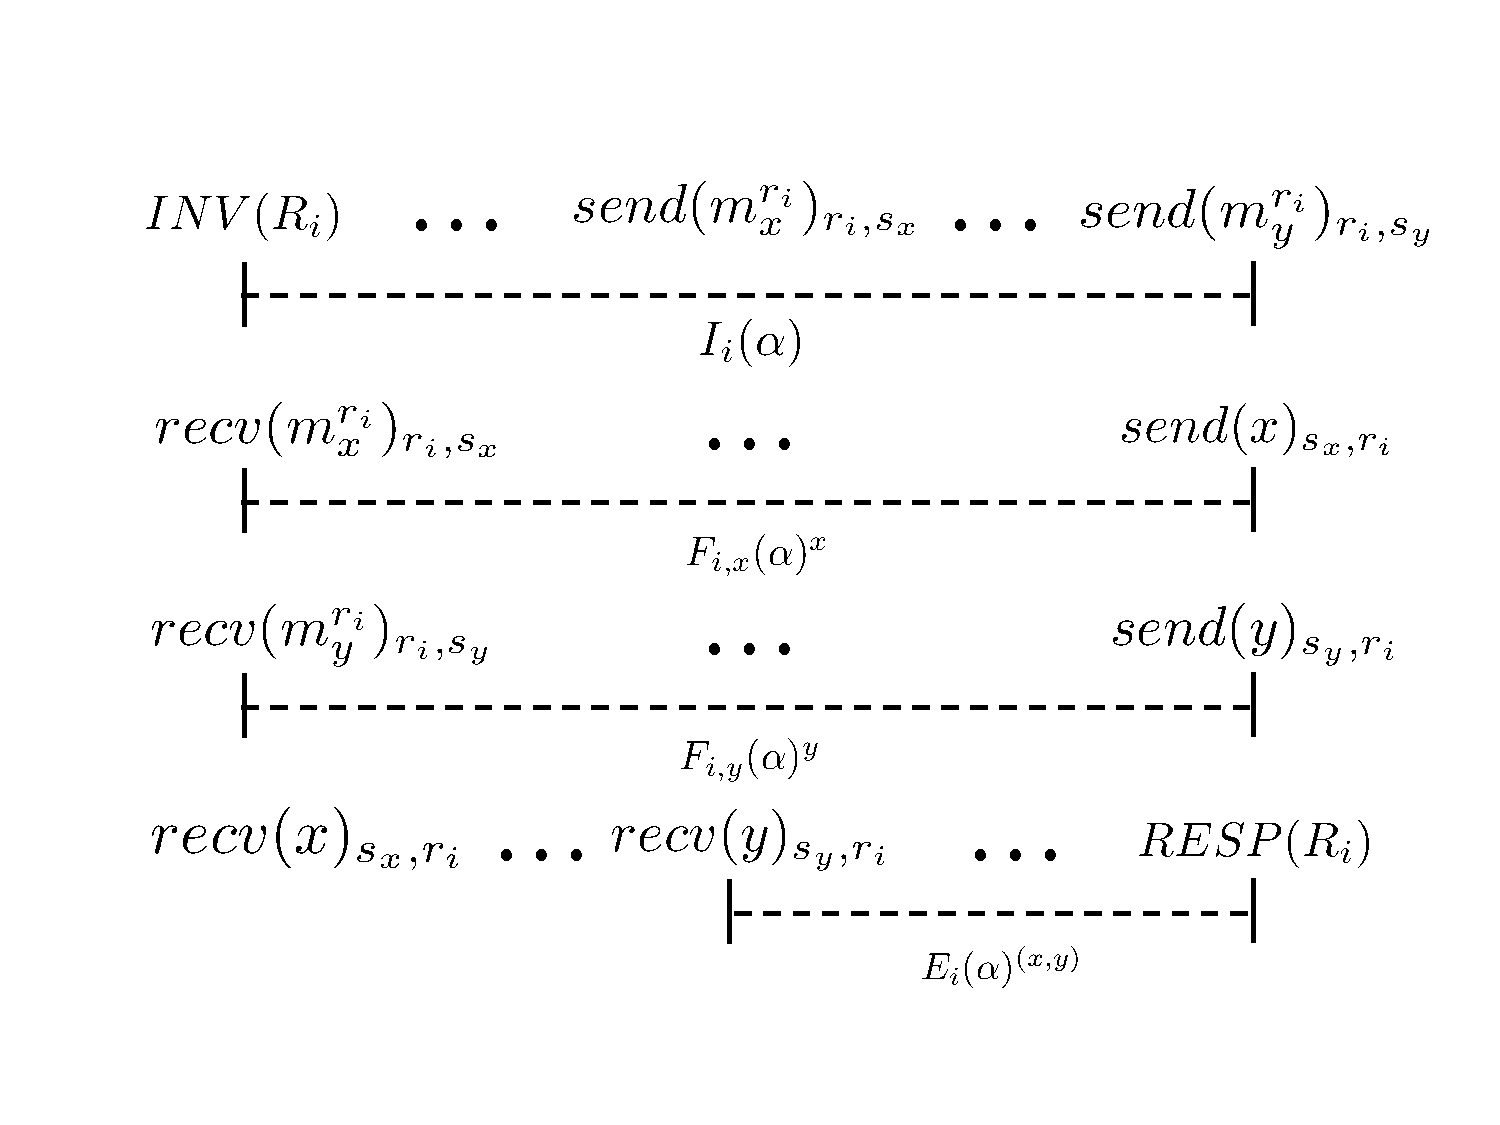
\includegraphics[scale=0.5]{figures/executions_3_2.pdf}
         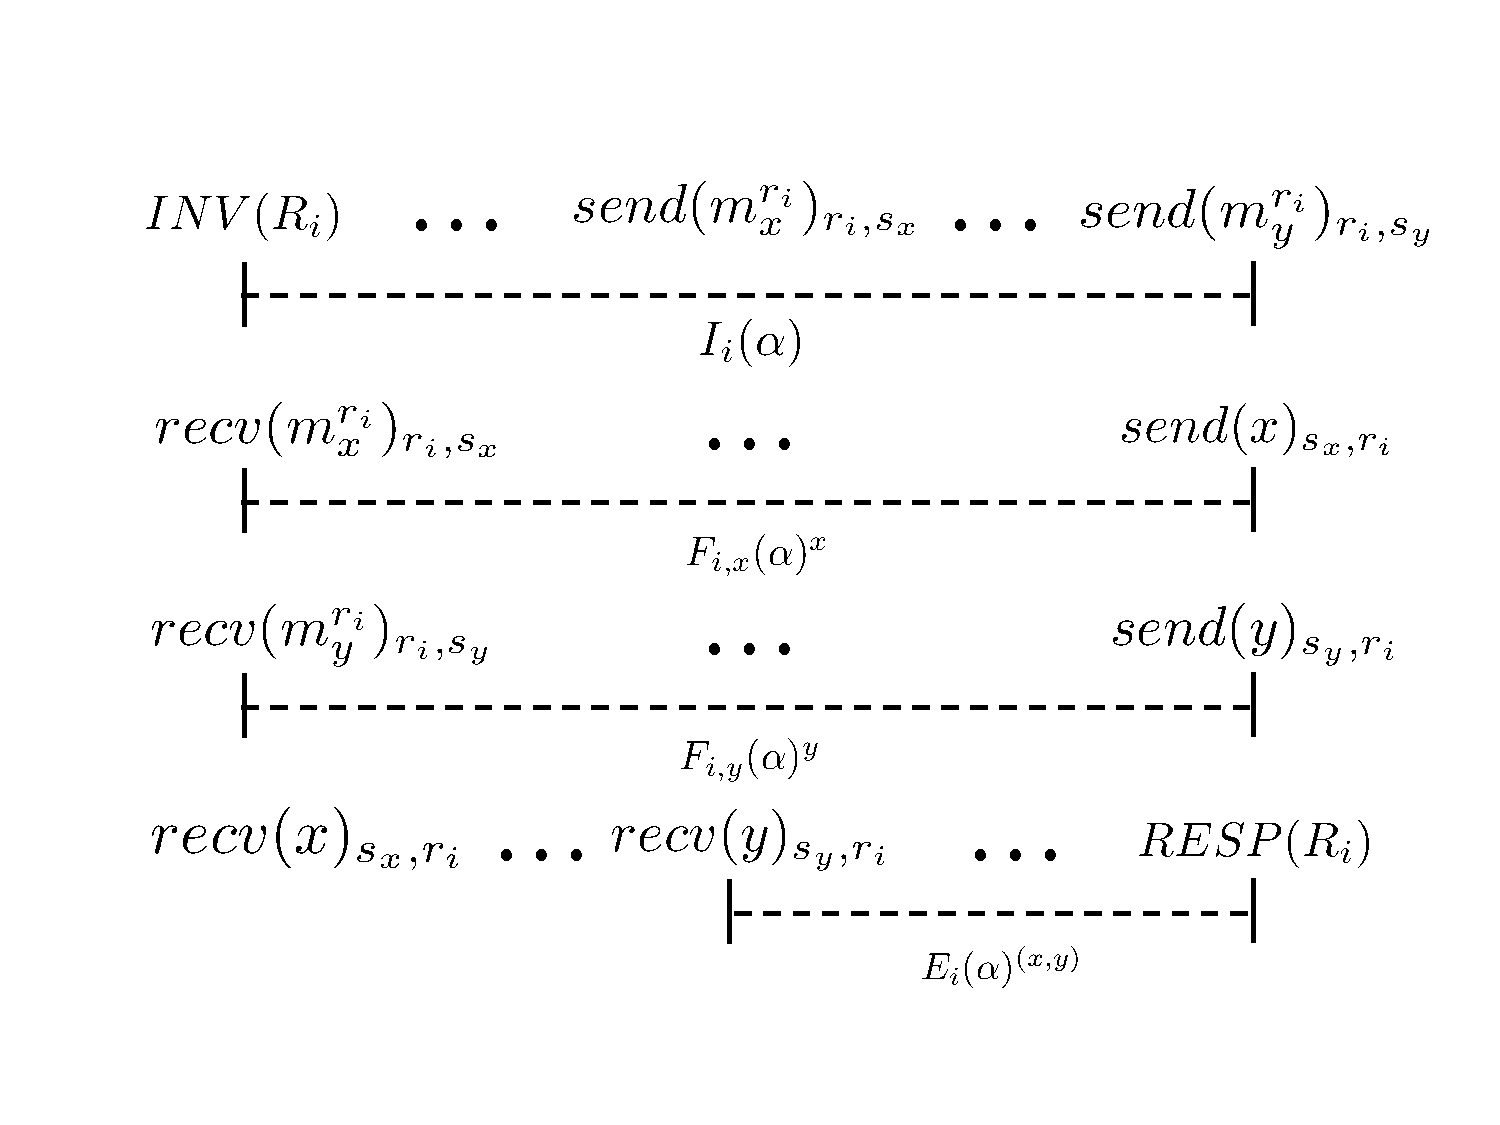
\includegraphics[width=4in]{figures/executions_3_2.png}
         \caption{
\small{The relevant actions in the execution fragments $I_i(\alpha)$, $F_{i,x}(\alpha)^{x}$,    $F_{i,y}(\alpha)^{y}$ and   $E_{i}(\alpha)^{(x,y)}$ for any \rot{} $R_i$, $i \in \{1, 2\}$
of a fair execution $\alpha$ of $\mathcal{A}$.}}
         \label{fig:exe3_fragments}
 \end{figure}
}

In our proofs, we frequently use arguments that rely on the existence of   non-blocking fragments and the constraints of strict serializability and write isolation. We derive the following use lemmas. In these lemmas, all \rots{} are assumed to have all SNOW properties, and we will derive contradictions in our main proofs. Due to space constraints, we explain these lemmas at a high level. %The proofs of these lemmas can be found in Appendix~\ref{app:lem_exec3_consistent}.

%We construct executions using \rots{} and \wots{} that always contact both servers $s_x$ and $s_y$.
%Because there is only one writer this makes objects $o_1$ and $o_2$ progress through versions together.
%This progression and strict serializability ensure that any \rot{} $R$ always returns the same version from both servers, e.g., $x_1$ and $y_1$.

%\wl{I'm not sure the purpose of the below paragraph now. Can we cut it out and just say the proof of the lemma is in the appendix? (I've cut it, but please confirm that's okay)}

%% Any  \rot{} $R$ initiated at a reader $r$, via the  
%% invocation action  $\INV{R}$ at $r$, after which the  actions $send(m_1^{r})_{r, s_x}$ and $send(m_2^{r})_{r, s_y}$, at $r$, send message $m_1^r$  to $s_x$ and $m_2^r$ to $s_y$, respectively. Once
%% $s_x$   receives $recv(m_1^{r})_{r, s_x}$  then  $s_x$ responds to $r$,  in a 
%% non-blocking manner,  with value $x$ via  action $send(x)_{s_x, r}$. Similarly,  after $s_y$  receives $m_2^{r}$ it  responds with $y$ to 
%% $r$ in a non-blocking manner via the action $send(y)_{s_y, r}$. After  $r$ receives $x$ and $y$ via actions $recv(x)_{s_x, r}$ and $recv(y)_{s_y, r}$, respectively,  $R$  completes
%%  with the response action $\RESP{R}$ and  returns $(x, y)$. 
%%
%% From the above discussion we can derive a lemma, which states in any  execution of $\mathcal{A}$,  if 
%% a server $s_i$  responds with a value $v_i$ during a   
%% \rot{}  then the \rot{} returns  
%% $v_i$ for  object $o_i$ and also, the pair of values $(x_t, y_t)$ are from some version $t$.
%% The result follows from the reliable channel model, where messages  reach at their destinations unaltered;  and by the S property  the object values, for objects $o_1$ and $o_2$,  returned by $R$  are of the same version.
%%
%% \wl{My cut of that paragraph ends here}
%%




%From the above discussion, it is easy to see that for any fair execution of $\mathcal{A}$ where $R_i$ is invoked, the adversary can always induce a fair execution of $\mathcal{A}$ where the fragments $I_i$, $\frage{F_{i,1}}{}{}$, $\frage{F_{i, 2}}{}{}$ and $E_i$ appear consecutively.
%Similarly, for any fair execution of  $\mathcal{A}$ where $R_2$ is invoked the adversary can always induce a fair execution of $\mathcal{A}$ where the fragments $I_2$, $\frage{F_{2,1}}{}{}$, $\frage{F_{2, 2}}{}{}$ and $E_2$ appear
  
%From this observation we can derive a lemma, which states in any execution of $\mathcal{A}$,  if 
%a server $s_i$ responds with a value $v_i$ during a   
%\rot{}  then the \rot{} returns  
%$v_i$ for  object $o_i$ and also, the pair of values $(x_t, y_t)$ are from some version $t$.
%The result follows from the reliable channel model, where messages reach at their destinations unaltered;  and by the S property  the object values, for objects $o_1$ and $o_2$,  returned by $R$  are of the same version.
The following lemma  proves that a \rot{} has to return the same version from both servers in order to satisfy strict serializability and write isolation.

\begin{lemma}\label{lem:exec3_consistent} 
Suppose $\alpha$ is any execution of $\mathcal{A}$ such that \rot{} $R$ is in $\alpha$. Suppose the  execution fragment $\frage{I}{\alpha}{} \circ \frage{F_{x}}{\alpha}{x_{t}} \circ \frage{F_{y}}{\alpha}{y_{s}} \circ \frage{E}{\alpha}{x_{t'}, y_{s'}}$ in $\alpha$, corresponds to $R$,  where   $x_t, x_{t'} \in V_1$ and  $y_s, y_{s'} \in V_2$, 
%then $(i)$ $s = s'$  and $ t=t'$ and $(ii)$ $s'=t'$.  
then $s=s'=t=t'$.  
%Similarly, if  the execution fragment $\frage{I_1}{\epsilon}{} \circ \frage{F_{2,1}}{\epsilon}{x} \circ \frage{F_{2,2}}{\epsilon}{y} \circ \frage{E_1}{\epsilon}{x', y'}$ appears, where   $x, x' \in V_1$ and  $y, y' \in V_2$, then $x = x'$ and $y=y'$.
\end{lemma}


%\wl{the removed proofs should all have pointers to their real proofs in the appendix, e.g., ``Proof given in Appendix~\ref{app:lem_exec3_consistent}''}

\remove{
\begin{proof}
Suppose $R$ is invoked at reader $r$.  Then, via the action $send(x_t)_{s_x, r}$, in 
execution fragment  $\frage{F_{1}}{\alpha}{x_{t}}$, server $s_x$ sends the value $x_t$ to $r$,   which is received at $r$ through the action 
$recv(x_{t'})_{s_x, r}$ in $\frage{E}{\alpha}{x_{t'}, y_{s'}}$.
 By the assumptions of the reliable channel automata in our model,  we have $x_{t}=x_{t'}$, i.e., $t=t'$. Similar argument for 
$\frage{F_{2}}{\alpha}{y_{s}}$  and $\frage{E}{\alpha}{x_{t'}, y_{s'}}$ leads us to conclude $s=s'$. Next, $R$ responds with $(x_{t'}, y_{s'})$, which implies  by the S property for executions of
 $\mathcal{A}$ that  $x_{t'}$ and $y_{s'}$ must correspond to the same version, i.e., $s'=t'$. %Therefore, we have $s = s' = t=t'$.
\end{proof}
}

%Note that the above results hold even if there are any other  execution fragments, that do not contain any actions at $r$, $s_x$ or $s_y$,   in-between the $I$, $F_i$ and $E$ execution  fragments. 

\remove{
\begin{corollary}\label{lem:exec3_consistent_corollary} 
Suppose $\alpha$ is any execution of $\mathcal{A}$ such that a \rot{} $R$ is in $\alpha$. Suppose the  execution fragment $\frage{I}{\alpha}{} \circ  X_1 \circ \frage{F_{1}}{\alpha}{x^{t}} \circ X_2 \circ  \frage{F_{2}}{\alpha}{y_{s}} \circ X_3 \circ \frage{E}{\alpha}{x_{t'}, y^{s'}}$ in $\alpha$,  corresponds to $R$,  where   $x_t, x_{t'} \in V_1$ and  $y^s, y^{s'} \in V_2$, $X_1, X_2, X_3$ are some execution fragments that do not contain any action at $r$, $s_x$ or $s_y$, and $s, s', t, t' $ are version identifiers  then $(i)$ $s = s'$  and $ t=t'$ and $(ii)$ $s'=t'$.  
\end{corollary}


\begin{proof} 
The constraint $(i)$ in the statement can be derived  from the fact that $\mathcal{A}$ satisfies the O property,  which implies that any version returned by $R$ for object value $o_1$ (or $o_2$) and this  must be the only version sent by the server $s_x$ (or $s_y$) to $r$. Constraint 
$(ii)$ from the S property of $\mathcal{A}$.
\end{proof}
}

%The following lemma states that new fair executions of $\mathcal{A}$ can be created by swapping execution fragments that  
%\blue{
%either $(a)$ have no input actions or 
%$(b)$ one of the fragments have no external (input or output) actions,
%}
% and in which   each fragment contains 
%actions that occur  only at one automaton and the automata for the two fragments are different. 
The following lemma states that we can create a new execution $\alpha'$ that is indistinguishable to $\alpha$ by swapping two fragments, which happen on two distinct automata in $\alpha$ if either $(a)$ both fragments have no input actions or 
$(b)$ one of the fragments have no external (input or output) actions. Our proofs leverage this lemma to create new executions by swapping such fragments and finally derive an execution that violates strict serializability.  
  \begin{lemma}[Commuting fragments] \label{lem:exec3_commute} 
  Let $\alpha$ be an execution of $\mathcal{A}$. Suppose $\frage{G_1}{\alpha}{}$ and $\frage{G_2}{\alpha}{}$ are any  execution fragments in $\alpha$ such that
  all actions in each fragment occur only at one automaton and  either $(a)$ none of the fragments contain input actions, or $(b)$ 
  at least one of the fragments have no external actions. Suppose $\frage{G_1}{\alpha}{}$ 
  and $\frage{G_2}{\alpha}{}$  occur at two distinct automata and the execution
  fragment $\frage{G_1}{\alpha}{}\circ \frage{G_2}{\alpha}{}$ occurs in $\alpha$.
  Then there exists an execution $\alpha'$ of $\mathcal{A}$, where  the execution fragment  $\frage{G_2}{\alpha}{}\circ \frage{G_1}{\alpha}{}$ appears in $\alpha'$, such that 
  %\blue{
  $(i)$  $\frage{G_1}{\alpha}{} \sim \frage{G_1}{\alpha'}{}$ and  $\frage{G_2}{\alpha}{} \sim \frage{G_2}{\alpha'}{}$
  %}
  $(ii)$ 
the prefix  in $\alpha$  before  $\frage{G_1}{\alpha}{} \circ \frage{G_2}{\alpha}{}$
 is identical to the prefix  in $\alpha'$ before  $\frage{G_1}{\alpha'}{} \circ \frage{G_2}{\alpha'}{}$; and $(ii)$ 
the suffix in $\alpha$  after   
 $\frage{G_1}{\alpha}{} \circ \frage{G_2}{\alpha}{}$
is identical to the suffix in $\alpha'$ after the execution fragment 
 $\frage{G_2}{\alpha'}{} \circ \frage{G_1}{\alpha'}{}$. 
 % Similar results  hold for the traces of $\alpha$ and $\beta$  in terms of the 
 %trace fragments   $\fragt{G_1}{\alpha}{}$ and $ \fragt{G_2}{\alpha}{}$
  \end{lemma}
 \remove{
  \begin{proof}
  This is clear because the adversary can move the actions in $G_2$ to occur before $G_1$ at their respective automata, and  because 
   either $(a)$ none of the fragments have any input action or $(b)$ at least one of them has no external actions, and hence 
  the actions in one of these fragments cannot affect the actions in the other fragment.
  \end{proof}
}


%The following lemma states that if there are two fair executions of $\mathcal{A}$ with a \rot{}  $R$ in each of them, and suppose at any server the non-blocking execution fragments  of $R$  are identical (in terms of the sequence of states and actions)  then in both executions, $R$   returns the same object value.
The following lemma states that if there are two fair executions of $\mathcal{A}$ with \rot{} $R$ in each of them, and suppose at any server the non-blocking fragments of $R$ are identical (in terms of the sequence of states and actions), then $R$ returns the similar values in both executions.
\begin{lemma}[Indistinguishability]  \label{lem:exec3_equiv}
Let $\alpha$ and $\beta$ be executions of $\mathcal{A}$ and let $R$ be any \rot{}. Then 
$(i)$  if $\frage{F_{x}}{\alpha}{} \stackrel{s_x}{\sim}\frage{F_{x}}{\beta}{}$ then both 
$R(\alpha)$ and $R(\beta)$ respond with the same value $x$ at $s_x$; and 
$(ii)$ if  $\frage{F_{y}}{\alpha}{} \stackrel{s_y}{\sim}\frage{F_{y}}{\beta}{}$ then both 
$R(\alpha)$ and $R(\beta)$ respond with the same value $y$ at $s_y$.
\end{lemma}


\remove{
\begin{proof}
Suppose $R$ is invoked at some reader $r$. Let $j \in \{1, 2\}$ and  suppose the fragments  $\frage{F_{j}}{\alpha}{}$ and  $\frage{F_{j}}{\beta}{}$ 
appears in $\alpha$ and $\beta$ respectively, where in $\frage{F_{j}}{\alpha}{}$ server $s_j$
sends  $v_j \in V_j$ to $r$. Then $R(\alpha)$ must return $v_j$ for object $o_j$ by the O property  of $\mathcal{A}$. Then since $\frage{F_{j}}{\alpha}{} \stackrel{s_j}{\sim} \frage{F_{j}}{\beta}{}$ then
in  $\frage{F_{j}}{\beta}{}$  the server $s_j$ 
must also  send $v_j$ to $r$,  therefore,  both $R(\alpha)$ and $R(\beta)$ must return value $v_j$ for $o_j$.
%Then by the $S$ property  $R(\beta)$ must return $(x_t, y_t)$, which proves the result of the lemma. 
%
\end{proof}
}


%Below we show that in any finite execution of $\mathcal{A}$ where the final action is an invocation of  \rot{} $R$ at a reader $r$, the adversary can always induce a fair execution of $\mathcal{A}$ where the fragments $I$, $\frage{F_{1}}{}{}$, $\frage{F_{2}}{}{}$ and $E$ appear consecutively in that order.
 The following lemma shows that for any finite execution of $\mathcal{A}$ that ends with the invocation of  \rot{} $R_1$, it is always possible to have an execution of $\mathcal{A}$ where the fragments $I$, $\frage{F_{x}}{}{}$, $\frage{F_{y}}{}{}$ and $E$ appear consecutively due to the asynchronous network.
\begin{lemma}\label{lem:read_format}
%If a \rot{} $R_i$ is invoked in $\mathcal{A}$ then there exists a fair execution $\epsilon$ of $\mathcal{A}$ such that 
%the fragments $\frage{I_i}{\epsilon}{}$, $ \frage{F_{i, 1}}{\epsilon}{x}$, $\frage{F_{i, 2}}{\epsilon}{y}$ and 
 %$\frage{E_i}{\epsilon}{x, y}$ appear in $\epsilon$.
If any finite execution of  $\mathcal{A}$ ends with $\INV{R}$, for a \rot{} $R_1$ then there exists an extension $\alpha$ which is a fair execution of $\mathcal{A}$ and  is  of the form  
   $\frage{P}{\alpha}{} \circ\frage{I}{\alpha}{} \circ \frage{F_{1,x}}{\alpha}{x} \circ \frage{F_{1,y}}{\alpha}{y} \circ \frage{E}{\alpha}{x, y} \circ \frage{S}{\alpha}{}$, where $\frage{P}{\alpha}{}$ is the prefix and $\frage{S}{\alpha}{}$ denotes the rest of the execution. 
 \end{lemma}
 
 \remove{
 \begin{proof}
 Consider a finite execution of $\mathcal{A}$  that end with  $INV(R)$, which  occurs at some reader  $r$, 
then the  adversary  induces the execution fragment $\frage{I}{\alpha}{}$  by delaying all actions, except the internal and output actions at $r$, between 
the actions $\INV{R}$ and the later of the actions $send(m_1^{r})_{r, s_x}$ and $send(m_2^{r})_{r, s_y}$. Next, the adversary  
delivers $m_1^{r}$ at $s_x$ (via the action $recv(m_1^{r})_{r, s_x}$) and delays all actions, other than internal and output actions at $s_x$, until $s_x$ responds with $x$, via  $send(x)_{s_x, r}$; 
we identify this  execution fragment
 as $\frage{F_{1}}{\alpha}{x}$. Subsequently, in a similar manner, 
the  adversary  delivers the message  $m_2^{r}$ and delays appropriate actions to induce the execution fragment 
$\frage{F_{2}}{\alpha}{y}$. Finally, the adversary  delivers the values $x$ and $y$ to $r$ (via the events $recv(x)_{s_x, r}$ and $recv(y)_{s_y, r}$), 
and delays all actions at other automata until $R$ completes  with action $\RESP{R}$ by returning $(x, y)$.  As a result, we  arrive at a fair execution of $\mathcal{A}$ of the form
 $\frage{I}{\alpha}{} \circ \frage{F_{1}}{\alpha}{x} \circ \frage{F_{2}}{\alpha}{y} \circ \frage{E}{\alpha}{x, y} \circ \frage{S}{\alpha}{}$.
\end{proof}
}


\remove{
 \begin{figure}[t]
      \centering
         %\includegraphics[width=4.0in,  height=4in]{figures/executions_3_1-crop.pdf} 
        \includegraphics[scale=0.4]{figures/executions_3_1-crop.pdf} 
          %\vspace{-2.5em}
         \caption{
        \small{Executions of $\mathcal{A}$ with three clients and operations $W$, $R_1$ and $R_2$ leading to the contradiction of S in $\alpha_{10}$.
        Arrows show the transposition of execution fragments from the previous execution.
         % The external requests and responses  at the clients  to and from the end-users are represented as invocation and responses for the transaction.
         }} 
         \label{fig:executions3}
 \end{figure}
}

\begin{figure}[t]
	%\centering
	\hspace*{-0.0cm}

		\centering
	     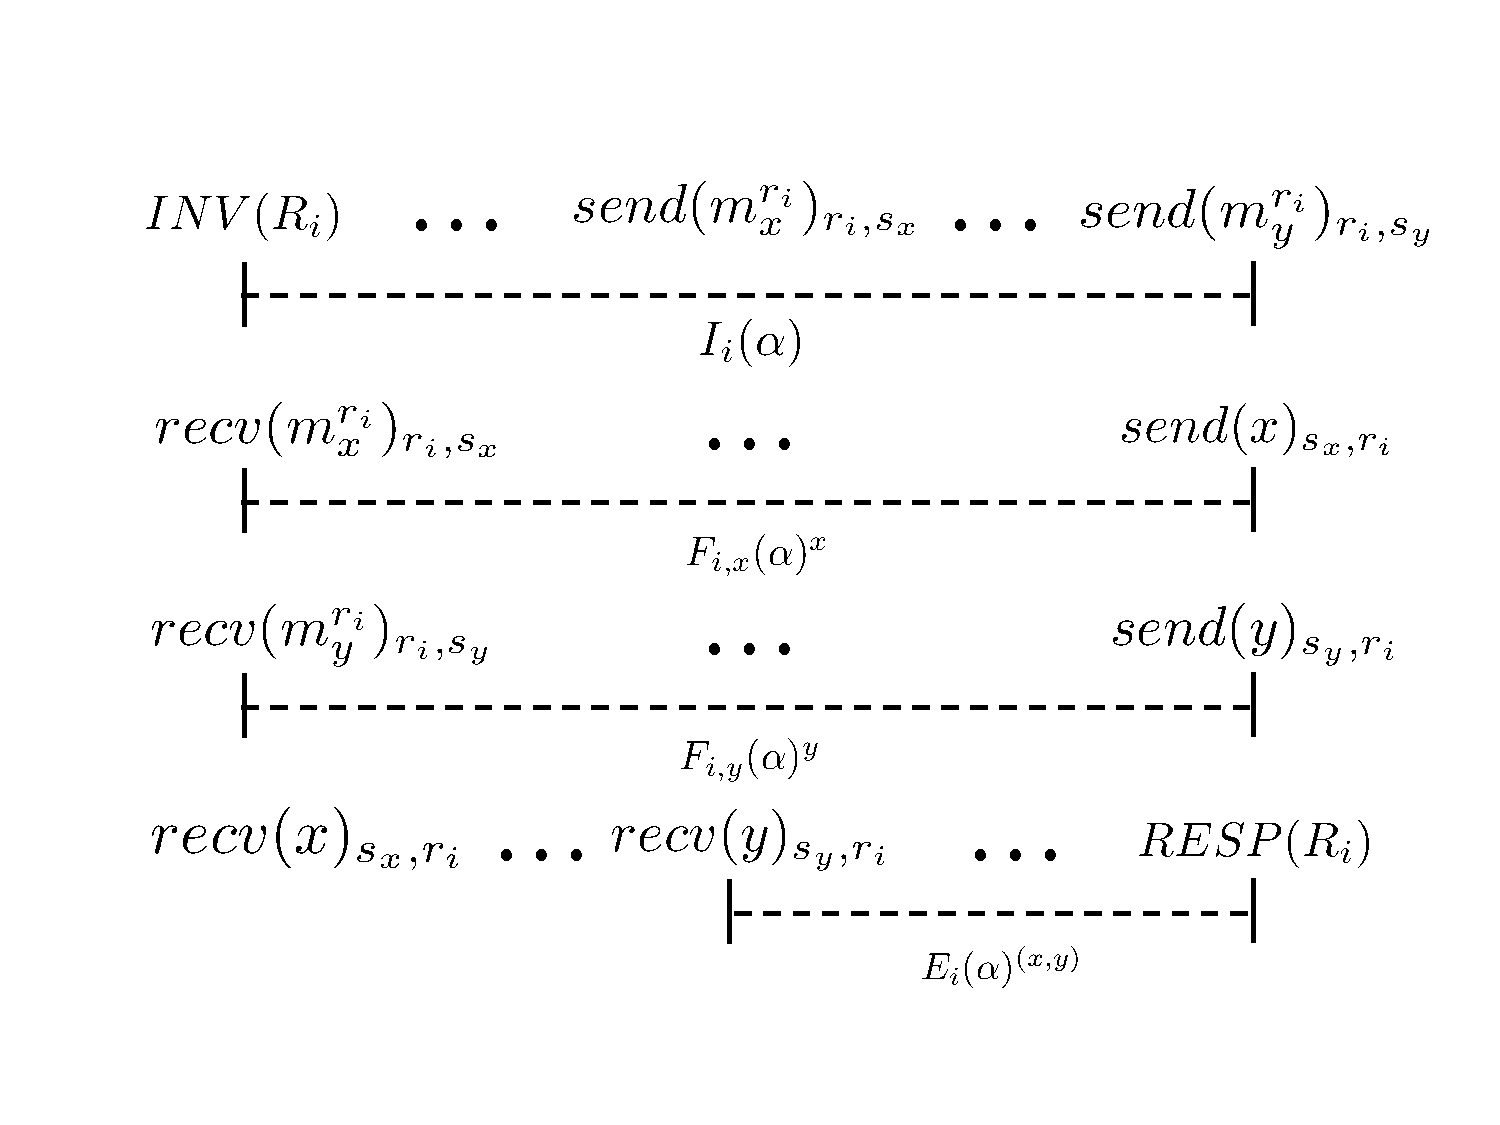
\includegraphics[width=3.0in]{figures/executions_3_2.pdf}
	     \caption{\small{
	      The relevant actions in the execution fragments $I_i(\alpha)$, $F_{i,x}(\alpha)^{x}$,    $F_{i,y}(\alpha)^{y}$ and   $E_{i}(\alpha)^{(x,y)}$ for any \rot{} $R_i$, $i \in \{1, 2\}$
			of a fair execution $\alpha$ of $\mathcal{A}$.
	     }}
	     \label{fig:exe3_fragments}
\end{figure}

\begin{figure}[t]
		\centering
		%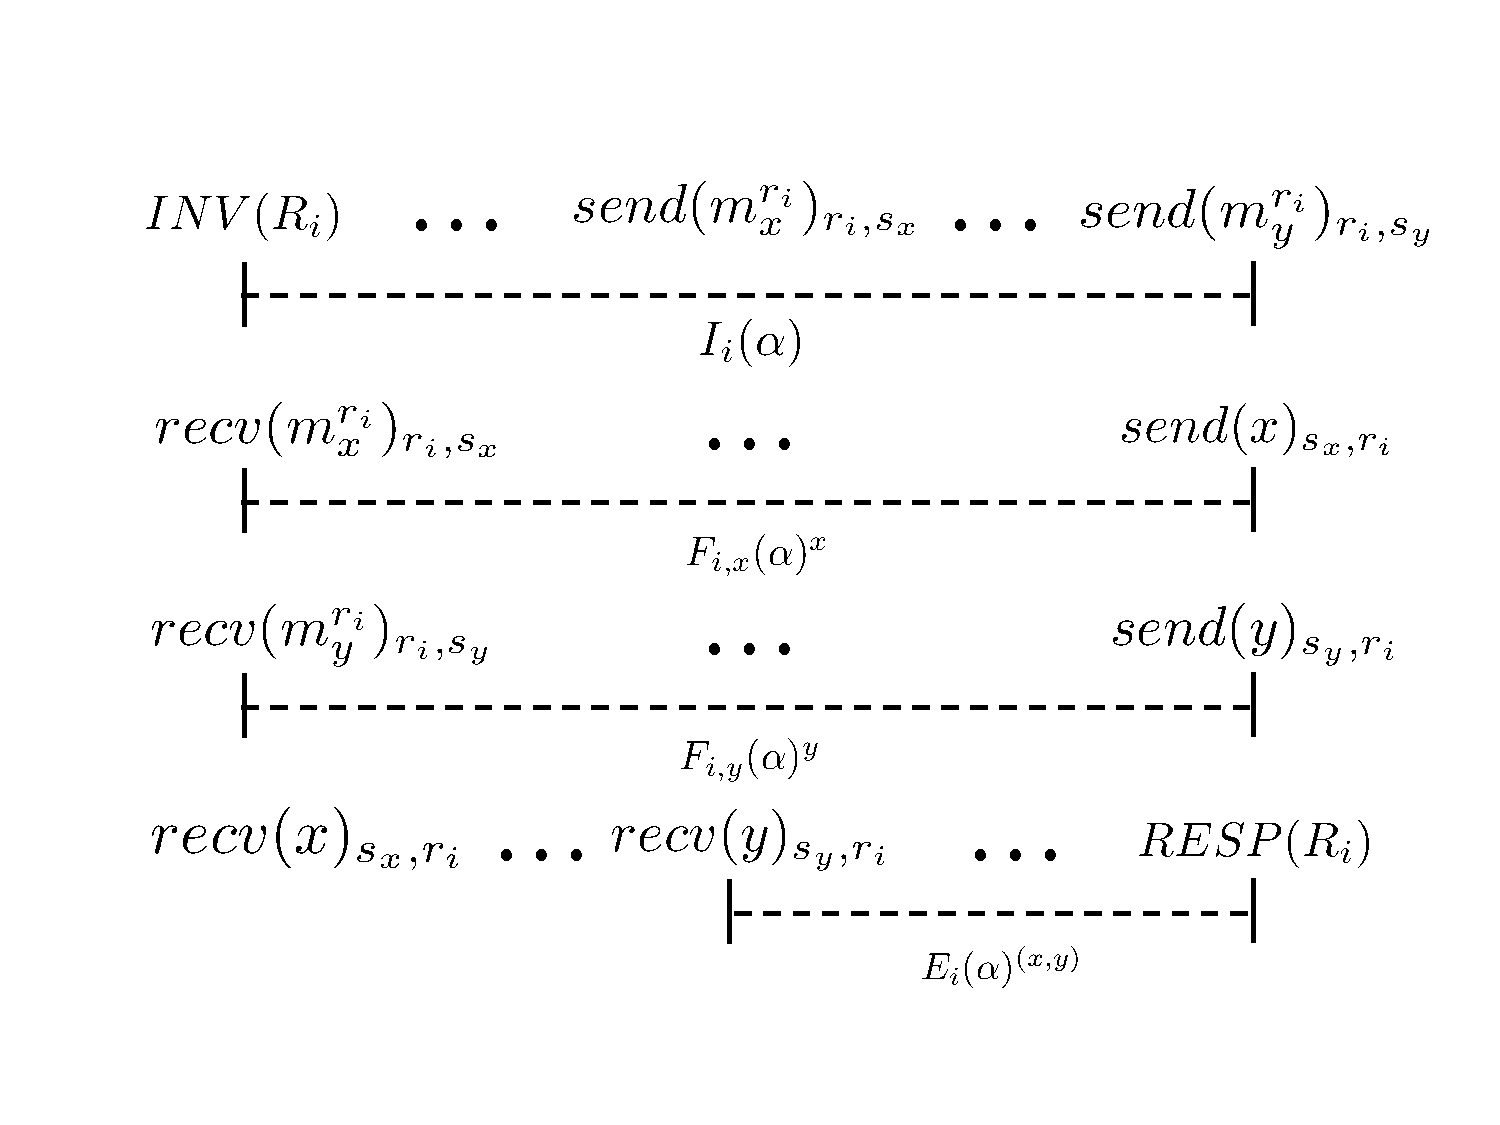
\includegraphics[width=3.2in]{figures/executions_3_2.pdf}		
		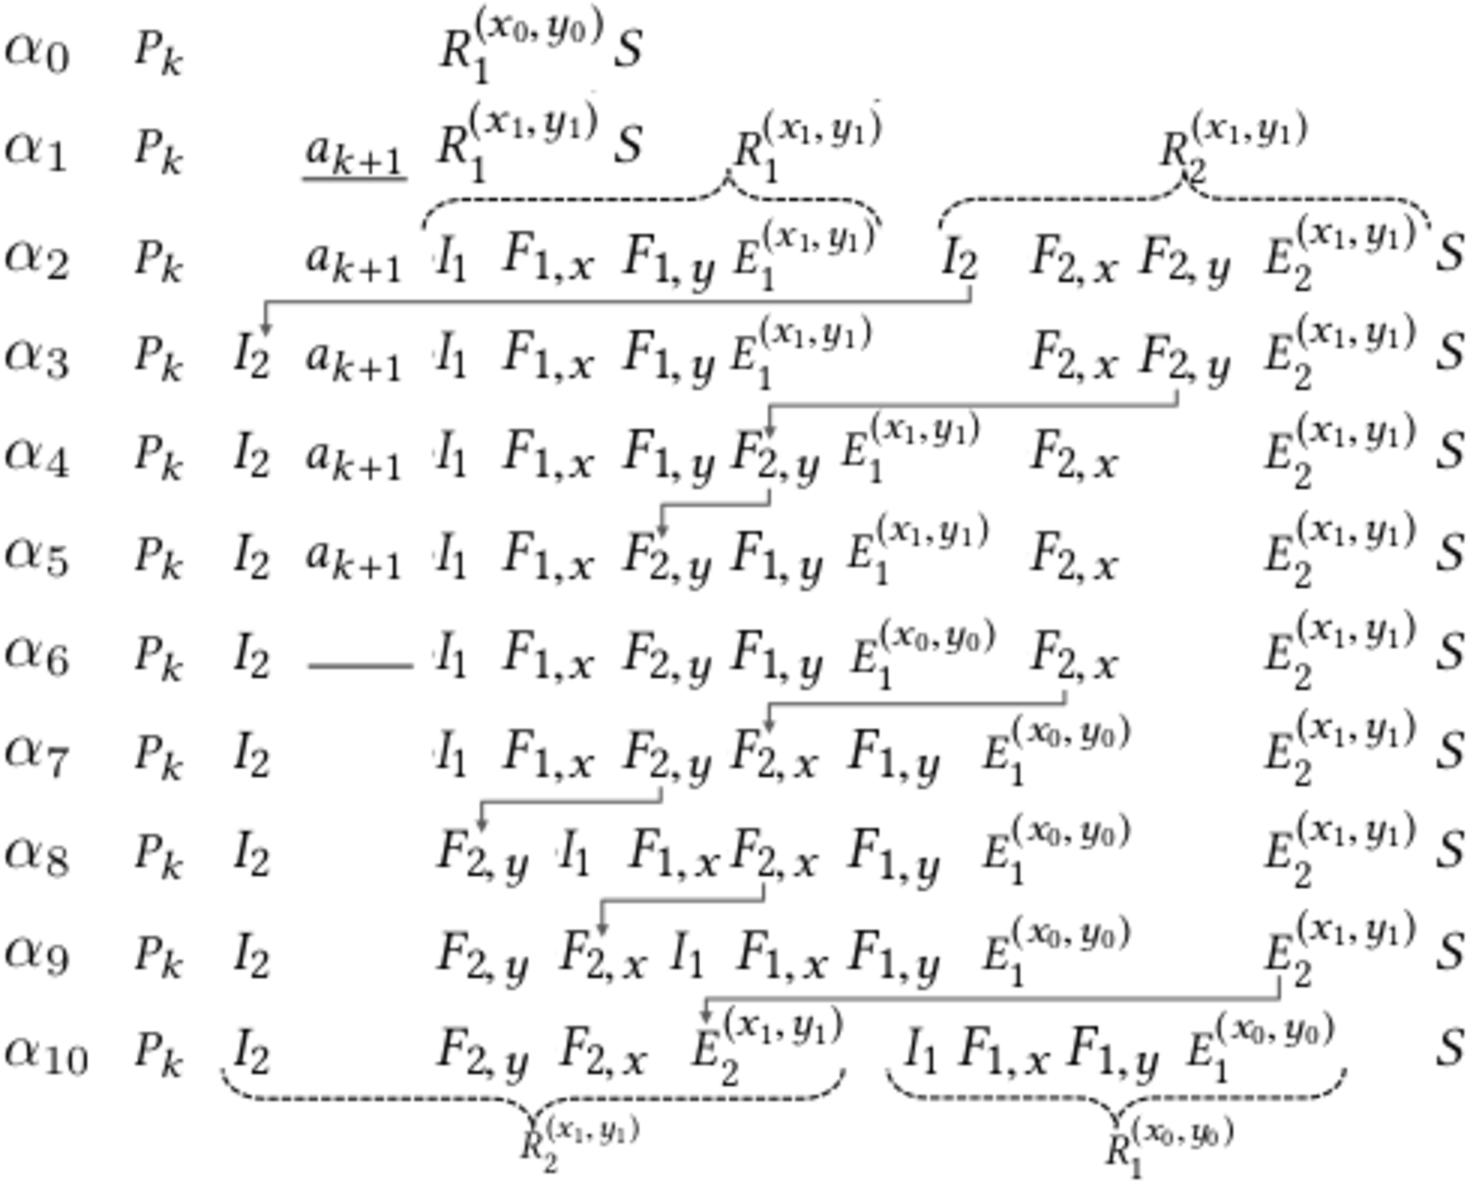
\includegraphics[width=3.0in]{figures/executions_3_1-cropa.pdf}		
		\caption{\small{Executions of $\mathcal{A}$ with three clients and operations $W$, $R_1$ and $R_2$ leading to the contradiction of S in $\alpha_{10}$.
			Arrows show the transposition of execution fragments from the previous execution.
		}}
           	\label{fig:executions3}	
%\label{fig:executions3}		 
\end{figure}
